\chapter{Asking Billionaires How They Got Rich (Houston)}

This chapter is not a blackboard derivation in the usual sense. It is an interview-driven lecture on the arithmetic of entrepreneurial scale, and so the mathematics appears here as a set of compact bookkeeping relations that make the spoken mechanism explicit. The host begins with spectacle---large names, large numbers, billion-dollar claims---and then resets the problem: how, in operational terms, do people build wealth at that scale, and what habits survive contact with real markets, real debt, real teams, and real risk?

\section{Headline Numbers and the Real Question}

The lecture opens with a teaser montage. We are given outcomes before causes, and the effect is deliberate. The cold open offers a few numerical anchors large enough to create curiosity:

\begin{align}
N_{\text{female founders}} &= 20,\\
\sum_{i=1}^{76} V_i &= \$1.27\ \text{billion},\\
\Pi_{\max} &= \$980\ \text{million}.
\end{align}

These are not yet explanations. They are the prologue quantities. Only after this burst of scale does the host reset in Houston at the Aspire Tour and tell us what the inquiry really is: we are here to interview entrepreneurs and operators in order to find the mechanisms behind such numbers.

That reset matters. The chapter should therefore begin as the lecture begins: first the spectacle of outcomes, then the analytical question. What produced these magnitudes? Was it initial capital, margins, investor support, systems, timing, negotiation, or some mixture of all of them?

\section{Kendra Scott and the Bootstrap Growth Loop}

The first full answer comes from Kendra Scott. The host moves rapidly from identity and industry to the large claim itself: a billion-dollar brand. But the interview becomes interesting only when the host asks for the mechanism, and Scott answers with a small beginning: the first collection was made with \$500.

We can write the bootstrap logic in the mildest possible algebraic form. Let \(C_t\) denote working capital at business cycle \(t\), let \(R_t\) be sales, let \(m_t\) be gross margin, let \(O_t\) be operating costs, and let \(B_t^{\text{serv}}\) be the servicing cost of the borrowing used to survive periods without outside equity. Then the spoken mechanism is summarized by

\begin{align}
C_0 &= \$500,\\
K_t^{\text{ext}} &\approx 0 \qquad \text{for roughly the first decade},\\
E_t &= m_t R_t - O_t - B_t^{\text{serv}},\\
C_{t+1} &= C_t + E_t.
\end{align}

This is not a literal lecture formula written on a board. It is the cleanest bookkeeping summary of what Scott describes: produce an initial collection, write orders, keep enough margin, reinvest, borrow when necessary, and continue.

\paragraph{Update rule.} At the first step the model says only this:
\begin{equation}
C_1 = \$500 + m_0 R_0 - O_0 - B_0^{\text{serv}}.
\end{equation}
The transcript gives us no numerical value for \(m_0\), nor for the costs. That is perfectly fine. The point is structural. Growth here is endogenous. If \(E_0>0\), the next cycle is larger; if \(E_0\leq 0\), the founder must either compress costs further, borrow more aggressively, or stop.

Scott adds two pieces that make the recurrence concrete. First, she says no investor would give her money for ten years. Second, she says she used credit-card debt, a line of credit, and collateralized everything she had. That means the recursion is not the fantasy
\[
C_{t+1}=C_t+\text{magic};
\]
it is the much harsher process in which retained earnings and debt service are always contending with one another.

\begin{figure}[h]
\centering
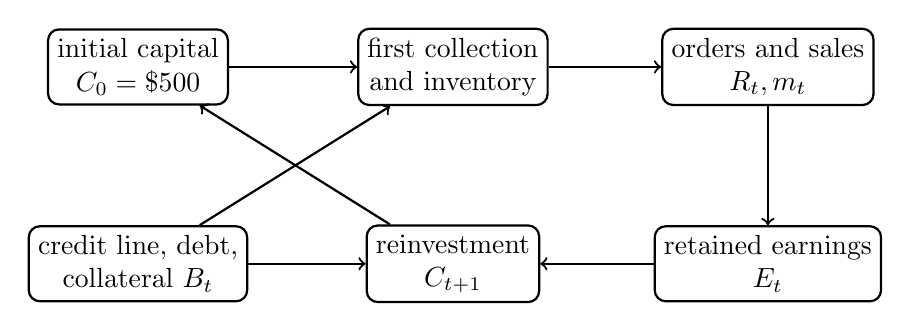
\begin{tikzpicture}[thick]
\node[draw, rounded corners, align=center] (c0) at (0,0) {initial capital\\\(C_0=\$500\)};
\node[draw, rounded corners, align=center] (prod) at (4,0) {first collection\\and inventory};
\node[draw, rounded corners, align=center] (sales) at (8,0) {orders and sales\\\(R_t,m_t\)};
\node[draw, rounded corners, align=center] (earn) at (8,-2.5) {retained earnings\\\(E_t\)};
\node[draw, rounded corners, align=center] (reinv) at (4,-2.5) {reinvestment\\\(C_{t+1}\)};
\node[draw, rounded corners, align=center] (debt) at (0,-2.5) {credit line, debt,\\collateral \(B_t\)};

\draw[->] (c0) -- (prod);
\draw[->] (prod) -- (sales);
\draw[->] (sales) -- (earn);
\draw[->] (earn) -- (reinv);
\draw[->] (reinv) -- (c0);
\draw[->] (debt) -- (prod);
\draw[->] (debt) -- (reinv);
\end{tikzpicture}
\caption{Editorial schematic of the bootstrap loop described in the Kendra Scott interview. The lecture did not supply a board figure; this diagram simply makes the spoken mechanism explicit.}
\end{figure}

There is also a delayed-capital phenomenon in the interview. The private-equity and venture-capital firms become interested only after the business generates visible demand---lines around the block, people coming in, traction that can no longer be ignored. In other words, outside capital arrives late, not early.

\subsection{Question \& Answer}

\paragraph{Question.} Why does profitable traction matter more than an impressive top line when outside capital is absent?

\paragraph{Answer.} Because the founder must propagate the business through actual cash generation, not through applause. Scott says this almost verbatim: build a profitable business, not merely one that looks good on the top line. In shorthand,
\begin{equation}
\text{top line} \not\equiv \text{healthy business},
\qquad
\mathrm{EBITDA}>0.
\end{equation}
The inequality is an editorial compression, but it captures the point faithfully. Revenue can impress; earnings keep the firm alive. Only after the business proves that it can convert activity into durable operating surplus do investors arrive in a meaningful way.

\section{Confidence, Preparation, and Negotiation}

Once the finance story is in place, the lecture turns to a second register. We move from cash mechanics to room mechanics. Scott is asked about the best advice she received from a mentor, and she rejects the lazy slogan that one must simply fake it until one makes it. The operative principle is sharper: do not be intimidated.

This part of the lecture matters because it keeps the notes from reducing entrepreneurship to a spreadsheet. The speaker is not saying that confidence replaces preparation. She is saying the opposite. Confidence is the behavioral form taken by preparation when one enters a room full of people who may try to dominate the terms.

The negotiation advice is especially precise. Scott says she comes in as a sponge, listens carefully, understands the other side's perspective, but never comes empty-handed. She has already done her homework. She knows who is in the room, what backgrounds they bring, what prior deals they have done, and what other people say about negotiating with them. In that sense, negotiation is treated not as theatrical aggression but as informed asymmetry. One wins by hearing, preparing, and then surprising.

The host then performs one of the lecture's characteristic recaps. He briefly turns to the audience and compresses the lesson into portable advice: go into the room prepared to win, regardless of who is on the other side. These recaps are not filler. They tell us how the lecture wants to be read.

\section{From One Business to Many: Systems and Scale}

The next pivot is abrupt on purpose. We leave the single-founder bootstrap case and encounter a private-equity operator who claims to have sold \(76\) companies for \(\$1.27\) billion in one year, and to run many businesses at once. The lecture is no longer about one brand compounding through reinvestment; it is now about the architecture of replication.

The key claim is that diversification is rational only after the operating process becomes portable. If we let \(P\) denote a common process, \(D\) a centralized data layer, \(M_i\) empowered managers, and \(L_i\) the individual business lines, then the lecture's systems thesis can be written as

\begin{align}
N_{\text{portfolio}} &= 86,\\
(P,D,M_i) &\Rightarrow \{L_i\}_{i=1}^{N}.
\end{align}

This is again editorial notation, not literal notation from the video. But it captures the operator's argument with some economy. The founder at the top is not manually re-inventing each company. He sees the whole through data, empowers people beneath him, and reuses the same process across different firms.

\subsection{Question \& Answer}

\paragraph{Question.} When does diversification become a rational extension of a system rather than a distraction from the core business?

\paragraph{Answer.} Only when the business already possesses a repeatable logic that can survive transplantation. The lecture states this plainly: focus on the actual system, and then the same process can apply to many things. In compressed form,
\begin{equation}
\text{replicable process} \Rightarrow \text{diversifiable operating model}.
\end{equation}
If the process is not stable, diversification multiplies confusion. If the process is stable, diversification becomes replication.

The same interview also introduces a contemporary industry claim: AI and tech are recommended because they offer the greatest opportunity for scale. The lecture does not formalize this claim, and neither should we. The important point is that scale appears here as a property of systems that can be extended, not merely of markets that are fashionable.

\section{Family Capital and the Interlude on Stewardship}

Midway through, the lecture takes an explicit detour. The host turns away from interviewing moguls and addresses the audience directly. This is a sponsor interlude, but it is not structurally meaningless. It changes the frame from enterprise capital to family capital.

The point is simple: learning to make money work for us is already one level of financial discipline, but there is another level in which we think about our children's future, long-term household planning, and the protection of the family balance sheet. The lecture also inserts a warning about trust---trust in people, employees, partnerships, and counterparties. The wording in the transcript is a little broken, but the intention is clear enough. Scale without judgment about trust becomes dangerous.

This section should remain brief in the final chapter, but it should not be erased. It changes the lecture's rhythm and broadens the meaning of stewardship.

\section{Marcus Lemonis and the Discipline of Substance}

Marcus Lemonis gives the lecture its cleanest discussion of fragility. He begins with industry selection: choose a field with white space and a clear consolidation opportunity. He says that twenty years earlier the relevant business was effectively at zero and later reached the level of a \(\$7\) billion business. In the notes we may summarize the scale claim as
\begin{align}
V_{\text{business}}(0) &\approx 0,\\
V_{\text{business}}(20\ \text{yr}) &= \$7\ \text{billion},
\end{align}
with the understanding that this is the speaker's own scale description, not an audited theorem.

The lecture then returns to the issue of teams. Delegation matters, but what matters more is surrounding oneself with people smart enough to challenge the founder. The logic is the same as before, but the emphasis is sharper. Scaling a company is not an exercise in protecting our ego; it is an exercise in constructing a decision environment in which better information can move upward.

Then comes the memorable distinction between substance and flash. What keeps people broke, Marcus says, is wanting to appear richer, stronger, or more powerful than they are. The deeper issue is not luxury itself but fragility. If we let total allocation be split into productive and performative pieces,
\begin{equation}
A = A_{\text{sub}} + A_{\text{flash}},
\end{equation}
then the lecture's risk claim may be compressed as
\begin{equation}
A_{\text{flash}} \uparrow
\qquad \Longrightarrow \qquad
\text{financial fragility} \uparrow.
\end{equation}

This is not a formal proof, but it is a faithful analytical rendering of the interview. Marcus's point is that lavish signals create a lifestyle with high fixed expectations. Once we live too high above our resilient baseline, every adverse decision becomes harder to survive. Buffett's old car and old house are invoked not as moral theater, but as examples of a life not organized around constant capital burn.

\subsection{Question \& Answer}

\paragraph{Question.} How do we enjoy success without making ourselves financially fragile?

\paragraph{Answer.} By refusing to confuse visible abundance with durable strength. The lecture's answer is not asceticism. It is balance. Nice things are not forbidden. What is forbidden, if we want resilience, is to let the symbolic layer of wealth consume the capital, habits, and psychological range that allow us to survive a downturn. The lecture puts this almost physically: every person is one decision away from losing a great deal, and the lower our necessary burn rate, the less catastrophic that loss becomes.

The host again recaps the lesson for the audience. He does not say merely that Lemonis delegated well. He says the scale came from surrounding oneself with people smarter than oneself and empowering them to make the right decisions.

\section{Timing, Health, Standards, and Value}

The closing movement condenses the lecture's themes into principles. Daymond John first reframes wealth through two maxims. The first is that money is a fine slave and a terrible master. The second is his line about pioneers and settlers. The point is timing. Originality by itself is not enough. If the market does not yet understand the product, the pioneer pays the price of being first; the settler may inherit the land once it becomes legible.

We can write the timing claim in its most compact form as
\begin{equation}
\text{too early} \Rightarrow \text{market does not yet understand the offer}.
\end{equation}

Daymond then answers a question about becoming a multimillionaire by changing the definition. If health is gone, the money no longer answers the real question. In other words, wealth is bounded above by the life that can actually make use of it.

Billy Ray Taylor closes the lecture differently. He gives us metaphors that are really standards. Trust your wings, not the branch. Be deliberately clear. You cannot manage a secret. Set the standard and do not widen home plate. Know your worth.

The home-plate analogy is not mathematics in the strong sense, but it is exact enough to matter: the plate is \(17\) inches in little league, in high school, and at higher levels too. The standard does not expand to accommodate weakness. This becomes his way of speaking about price, worth, and value proposition.

\subsection{Question \& Answer}

\paragraph{Question.} What is the difference between charging a price and stating a value proposition?

\paragraph{Answer.} The lecture's answer is given through a worked rhetorical example. Billy Ray says that free consulting and free software were neglected. When he attached a price and linked it to the client's loss and possible upside, the same offer became legible as an investment. If we write his arithmetic exactly as he states it, we obtain
\begin{align}
Y_{\text{Billy Ray}} &\in [\$1\text{M},\,\$3\text{M}],\\
\text{fee} &= \$5{,}000,\\
\text{claimed client gain} &= \$5{,}000{,}000,\\
\frac{\text{claimed client gain}}{\text{fee}} &= 1000.
\end{align}

This ratio is rhetorical, not audited. But that is enough for the lecture's point. A mere price sounds like cost; a framed value proposition sounds like asymmetric return. The entrepreneur is not simply naming a fee. He is teaching the client how to compare the fee with the outcome.

We also hear the phrase ``deliberate clarity'' and the line ``you can't manage a secret.'' That is an excellent summary of the entire closing segment. The lecture ends by tying wealth not only to scale and effort, but to explicit standards: standards of timing, standards of health, standards of worth, and standards of speech.

\section{Summary}

The lecture begins with giant quantities and ends with operating invariants. Along the way we move from bootstrap finance to investor timing, from confidence to preparation, from one company to a portfolio, from substance to flash, and from raw price to articulated value. If we compress the chapter into one sentence, it is this: durable wealth is not presented as a mysterious windfall, but as a sequence of disciplined recursions---capital into margin, margin into reinvestment, process into scale, scale into responsibility, and standards into staying power.